\documentclass[12pt,a4paper]{article}

\usepackage[margin=1in]{geometry}
\usepackage[T1]{fontenc}
\usepackage[utf8]{inputenc}
\usepackage{lmodern}
\usepackage{graphicx}
\usepackage{booktabs}
\usepackage[table]{xcolor}
\usepackage{array}
\usepackage{siunitx}
\usepackage{hyperref}
\usepackage{enumitem}
\usepackage{setspace}
\usepackage{titlesec}
\usepackage{float}

% image folder path
\graphicspath{{images/}}

\definecolor{PrimaryBlue}{HTML}{1E3A8A}
\definecolor{AccentBlue}{HTML}{2563EB}
\definecolor{SoftBlue}{HTML}{DBEAFE}
\definecolor{SoftGray}{HTML}{F3F4F6}
\definecolor{DarkText}{HTML}{111827}

\hypersetup{
    colorlinks=true,
    linkcolor=AccentBlue,
    urlcolor=AccentBlue,
    citecolor=AccentBlue,
    pdftitle={Quantum Path Finding Streamlit App Report},
    pdfauthor={Copilot}
}

\titleformat{\section}{\large\bfseries\color{PrimaryBlue}}{\thesection}{0.6em}{}
\titleformat{\subsection}{\normalsize\bfseries\color{AccentBlue}}{\thesubsection}{0.6em}{}

\setlist[itemize]{leftmargin=1.2em, itemsep=0.2em, topsep=0.2em}
\setlength{\parskip}{0.6em}
\setlength{\parindent}{0pt}
\renewcommand{\arraystretch}{1.2}

\newcommand{\placeholderfigure}[2]{%
\begin{figure}[h]
    \centering
    \fcolorbox{PrimaryBlue}{SoftBlue}{%
        \parbox[c][4cm][c]{0.9\linewidth}{%
            \centering\textbf{#1}\\[0.5em]
            \small #2
        }%
    }
    \caption{#1}
\end{figure}
}

\begin{document}

\begin{titlepage}
    \centering
    \vspace*{1.5cm}
    {\Huge\bfseries\color{PrimaryBlue} Quantum Path Finding Visualizer\par}
    \vspace{0.5cm}
    {\Large Project Report\par}
    \vskip 1.5cm
    {\large\color{DarkText} By \textbf{Abdullah Tariq}\par}
    \vspace{1.5cm}
    \begin{minipage}{0.85\textwidth}
        \setlength{\fboxsep}{14pt}
        \color{DarkText}
        \fcolorbox{PrimaryBlue}{SoftGray}{%
            \parbox{0.95\textwidth}{%
                This report summarizes the project structure, the path-finding algorithms used in the app, and the role of the quantum-inspired Grover approach. 
                It discusses how the grovers search algorithm works in the context of path finding and how it compares to classical methods.
                It contains the analysis of the results, including a comparison table and visual outputs from the app.
            }%
        }
    \end{minipage}
    \vfill
    {\large\today\par}
\end{titlepage}

\tableofcontents
\newpage

\section{Project Overview}
The project has a Streamlit front-end and a Python back-end that implements three path-finding algorithms: Breadth-First Search (BFS), A* Search, and a quantum-inspired Grover search.
The user can interact with the app to create a grid, place obstacles, and run the algorithms to find paths from a start node to an end node. 
Although I have provided random grid generation, the user can also manually edit the grid to create specific scenarios for testing. \\

The goal here is to compare the classical search methods (BFS and A*) with a quantum-inspired approach (Grover) in a way that is visually intuitive.
The app focuses on clarity and side-by-side comparison rather than on heavy technical complexity, making it suitable for educational purposes and for demonstrating the differences between classical and quantum-inspired search methods.

\section{System Structure}
The codebase is divided into clear parts:
\begin{itemize}
    \item \textbf{Grid management:} stores the board, start/end points, and obstacles.
    \item \textbf{Algorithms:} implements BFS, A*, and Grover-based path search.
    \item \textbf{Visualization:} renders the grid, highlights paths, and draws quantum plots.
    \item \textbf{UI layer:} handles the Streamlit layout, controls, and result display.
    \item \textbf{Utils:} contains helper functions for timing, metrics, and data formatting.
\end{itemize}

This structure keeps the app easy to maintain because each part has a specific responsibility.
It also allows for future extensions, such as adding more algorithms or improving the quantum visualization, without needing to overhaul the entire codebase.

\section{Algorithms}
\subsection{Breadth-First Search}
BFS is a standard graph search method. 
It explores the grid level by level, so it is guaranteed to find the shortest path in an unweighted grid if one exists. 
In this project, BFS acts as a simple and reliable baseline for comparison. \\

\noindent At first it was giving same path as the Grovers search given that it uses it so I changed it slightly to have an ordered exploration of the neighbors (e.g., always checking right, down, left, up) to ensure it produces a consistent path that can be compared with the other algorithms.

\subsection{A* Search}
A* is one of the best-known informed search algorithms. 
It combines actual distance traveled with a heuristic estimate of the remaining distance to the goal. 
In a grid, the Manhattan distance is a natural heuristic because movement is restricted to nearby cells.
A* is usually faster than BFS because it guides the search toward the target instead of exploring every direction equally. \\

\noindent This is well observed in the app, where A* typically explores fewer nodes than BFS, especially in larger grids with many obstacles.


\subsection{Grover Search}
Grover search is the quantum-inspired part of the project and is the most novel algorithm here. 
Unlike BFS and A*, which directly move through the grid, Grover search works on quantum states. 
It increases the probability of measuring a desired state by repeatedly amplifying it with Grover iterations. \\

\noindent In this app, Grover is used as a conceptual demonstration of how a quantum search process can support path finding. 
The algorithm is more experimental than BFS or A*, so the report should describe it as a new approach rather than a drop-in replacement for classical search.
It acts as local search where it finds the path accurately with way fewer node explored.

\subsubsection{Working of Grovers Algorithm}
Grover's algorithm is designed to search an unsorted database with $N$ entries in $O(\sqrt{N})$ time, which is a significant improvement over classical algorithms that require $O(N)$ time.
In the context of path finding, we can think of the grid as a search space where each cell represents a potential state.
Each cell here is encoded in a binary string, for example, in a $4 \times 4$ grid, we can represent each cell with a 4-bit binary string (e.g., $0000$ for the top-left cell, $1111$ for the bottom-right cell). \\

\noindent It encodes the number of qubits as $\lceil \log_2(N) \rceil$, where $N$ is the total number of cells in the grid.
It has $4$ major steps:
\begin{enumerate}
    \item \textbf{Initialization:} Start with an equal superposition of all possible states (cells).
    \item \textbf{Oracle:} Apply a quantum oracle that marks the target state
    \item \textbf{Diffusion Operator:} Apply the Grover diffusion operator to amplify the probability of the marked state.
    \item \textbf{Convergence:} Measure the final state and check if it matches the target.
\end{enumerate}

The algorithm iteratively applies the oracle and diffusion operator until it finds the target state with high probability.
This approach is particularly effective in large search spaces, making it an interesting choice for path finding in complex grids.
This is usually done in $O(\sqrt{N})$ iterations, which is a significant improvement over classical search algorithms that require $O(N)$ time.

\section{Visual Output}
The app shows the grid, the discovered path, and supporting plots.
For example, when run on a $8 \times 8$ grid, this is the grid produced alongside with the comparison of the algorithms and the grovers convergence plot.

\begin{figure}[H]
    \centering
    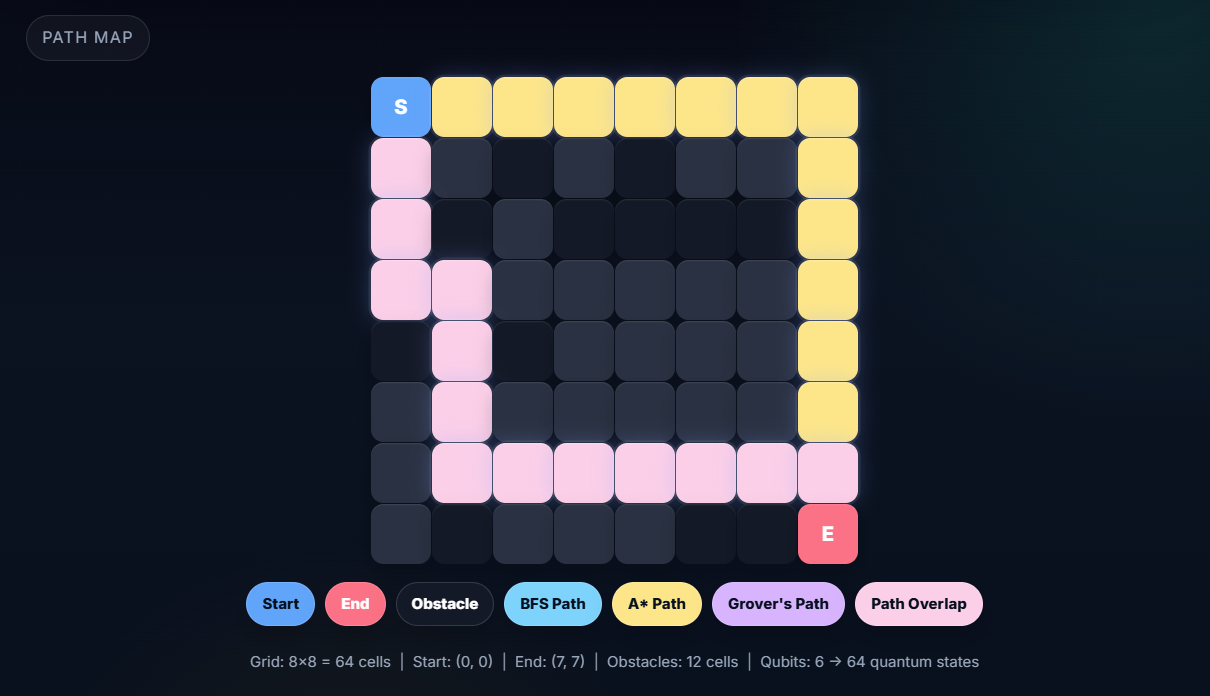
\includegraphics[width=0.8\textwidth]{Main_grid.png}
    \caption{Example of the grid visualization showing the start point, end point, and obstacles.}
\end{figure}

Then the side-by-side comparison of the algorithms is shown, where you can see the time they took, nodes explored, and path length.

\begin{figure}[H]
    \centering
    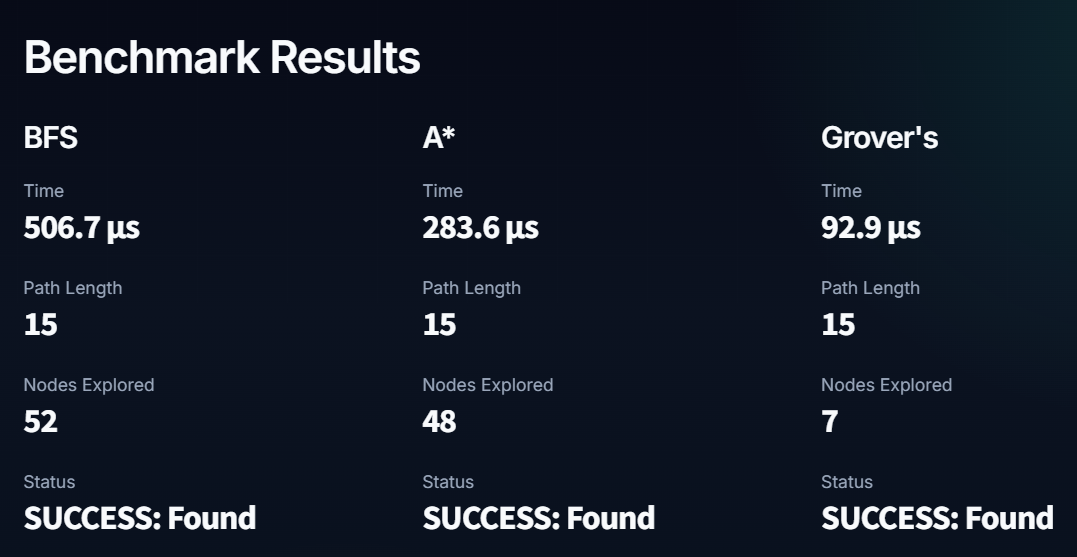
\includegraphics[width=0.8\textwidth]{Algorithm_comparison.png}
    \caption{Side-by-side comparison of BFS, A*, and Grover search results.}
\end{figure}

Finally, the Grover-related plot shows how the probability of finding the target state evolves with each iteration, demonstrating the quantum search process.

\begin{figure}[H]
    \centering
    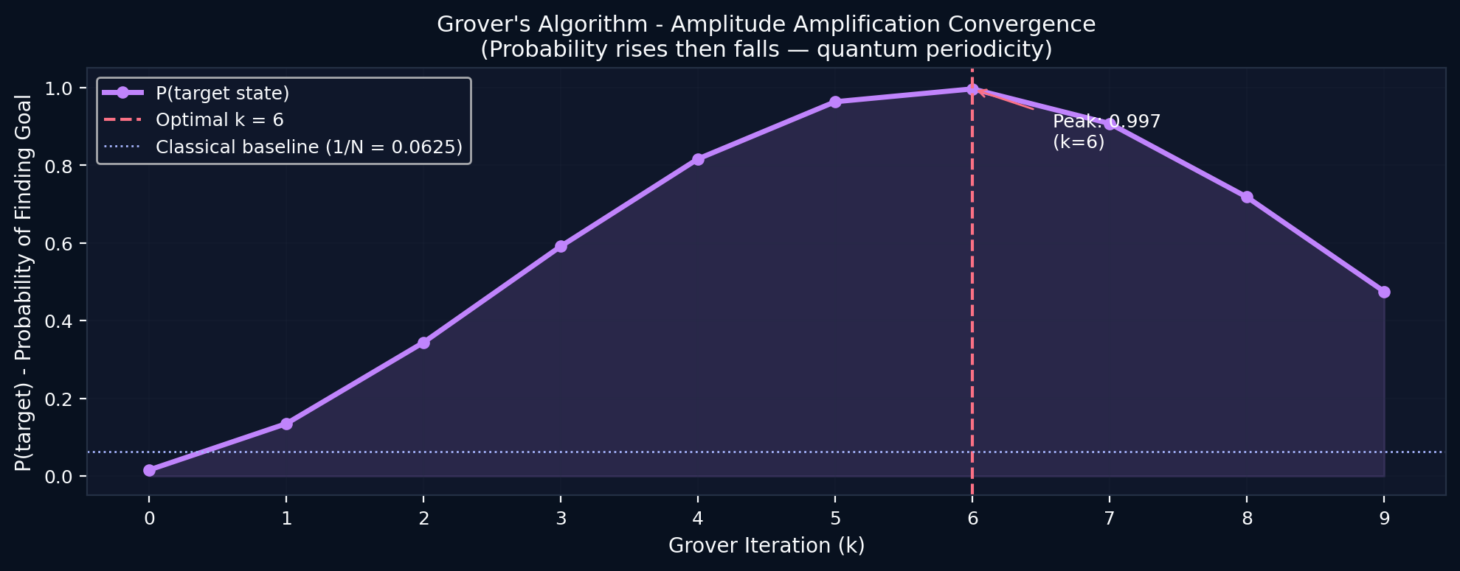
\includegraphics[width=0.8\textwidth]{Convergence.png}
    \caption{Grover's algorithm convergence plot showing the probability of finding the target state over iterations.}
\end{figure}

\section{Comparison Table}
This table summarizes the key metrics for each algorithm, including time taken, nodes explored, path length, and any relevant notes about their behavior in the context of this project.

\rowcolors{2}{SoftGray}{white}
\begin{table}[h]
\centering
\caption{Algorithm Comparison Summary for $n = 16$}
\begin{tabular}{>{\raggedright\arraybackslash}p{2.3cm} >{\centering\arraybackslash}p{2.2cm} >{\centering\arraybackslash}p{2.2cm} >{\centering\arraybackslash}p{2.2cm} >{\centering\arraybackslash}p{2.2cm} >{\raggedright\arraybackslash}p{3.6cm}}
\rowcolor{PrimaryBlue}
\color{white}\textbf{Algorithm} & \color{white}\textbf{Time (ms)} & \color{white}\textbf{Nodes Explored} & \color{white}\textbf{Path Length} & \color{white} \textbf{Efficiency} & \color{white}\textbf{Notes} \\
BFS & $985.7 \unit{\micro\second}$ & $199$ & $31$ & $0.1558$ & Baseline shortest-path search. \\
A* & $1.47 \unit{\milli\second}$ & $175$ & $31$ & $0.1771$ & Heuristic search using Manhattan distance. \\
Grover & $72.7 \unit{\micro\second}$ & $13$ & $31$ & $2.3846$ & Quantum-inspired search and path reconstruction. \\
\end{tabular}
\end{table}

\section{Implementation Notes}
A few implementation choices make the app easier to use:
\begin{itemize}
    \item The grid is editable so the user can place obstacles manually.
    \item The results are displayed in a consistent visual style.
    \item The UI separates input controls from output so the comparison is clear.
    \item The quantum visualizations are included as supporting material rather than as the main result.
\end{itemize}

\section{Conclusion}
This project provides a compact comparison between classical and quantum-inspired path finding. BFS offers a simple baseline, A* improves efficiency through heuristics, and Grover introduces a quantum-search perspective that makes the project more exploratory and research-oriented.

This table below summarizes the topics covered in this project and their relevance to the overall goal of demonstrating path finding algorithms in a visually intuitive way.
\begin{figure}[H]
    \centering
    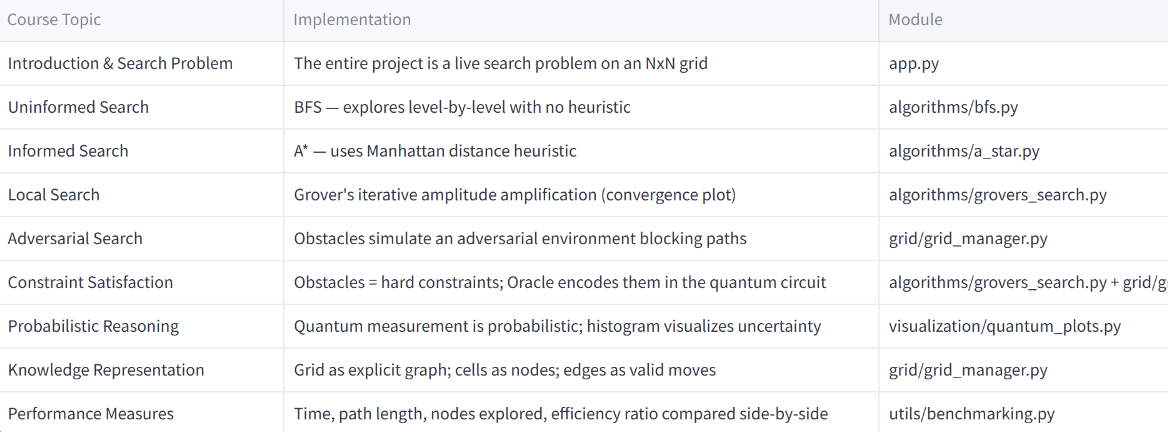
\includegraphics[width=1\textwidth]{Table.png}
    \caption{Topics covered in the project and their relevance to the overall goal.}
\end{figure}
\end{document}
